\documentclass[12pt]{standalone}

\usepackage{amssymb} 
\usepackage{amsmath} 

\usepackage[no-math]{fontspec}
\usepackage{unicode-math}
\setmainfont{TeX Gyre Heros}
\setmathfont{Stix Two Math}

\usepackage{xcolor}
\definecolor{myblue}{HTML}{CCDEE9}
\definecolor{bgcolor}{HTML}{F3F4F4}

\usepackage{tikz}
\usetikzlibrary{arrows.meta, backgrounds}

\begin{document}
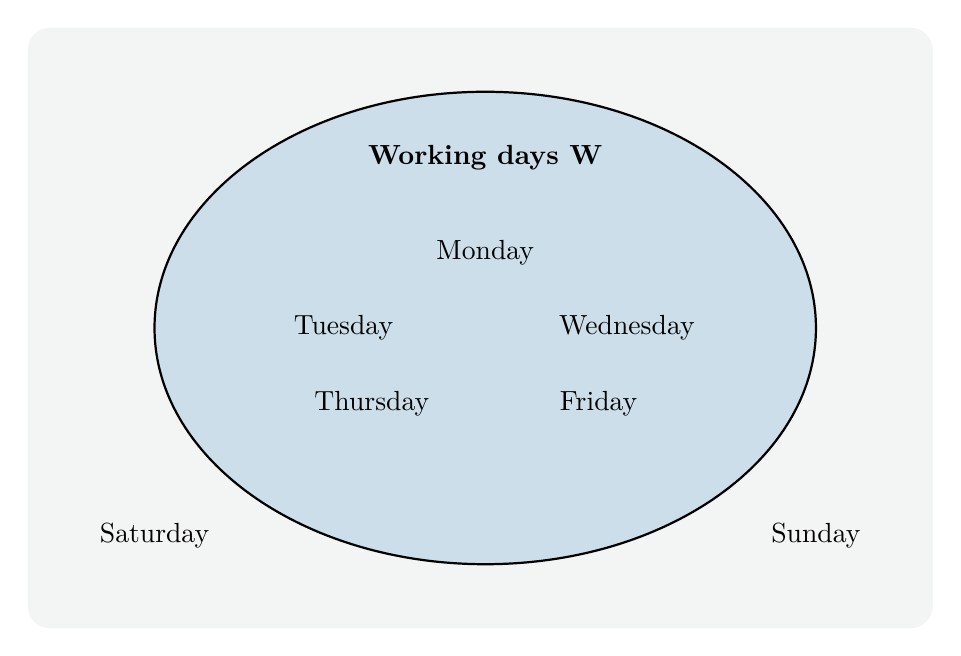
\begin{tikzpicture}[scale=1.2,
    show background rectangle,
    background rectangle/.style={fill=bgcolor, rounded corners=8pt},
    inner frame sep=0.8cm
]
  
  % Ellipse für Werktage
  \draw[thick, fill=myblue] (0,0) ellipse (3.5cm and 2.5cm);
  \node[font=\bfseries] at (0,1.8) {Working days $\mathbf{W}$};
  
  % Werktage innerhalb der Ellipse
  \node at (0,0.8) {Monday};
  \node at (-1.5,0) {Tuesday};
  \node at (1.5,0) {Wednesday};
  \node at (-1.2,-0.8) {Thursday};
  \node at (1.2,-0.8) {Friday};
  
  % Wochenende außerhalb der Ellipse
  \node at (-3.5,-2.2) {Saturday};
  \node at (3.5,-2.2) {Sunday};
  
\end{tikzpicture}
\end{document}